% !TeX root = ../../../thesis.tex

\chapter{DC Testbed Schematic}
\label{app:dc-test-bed-schematic}

In this chapter, the schematic of the DC testbed can be found in \autoref{fig:dc-test-bed-schematic}.
The relevant datasheets for parts used can be found in: \cite{2n3904-npn-transistor-datasheet} and \cite{bc556-pnp-transistor-datasheet}.

\begin{figure}[htb]
	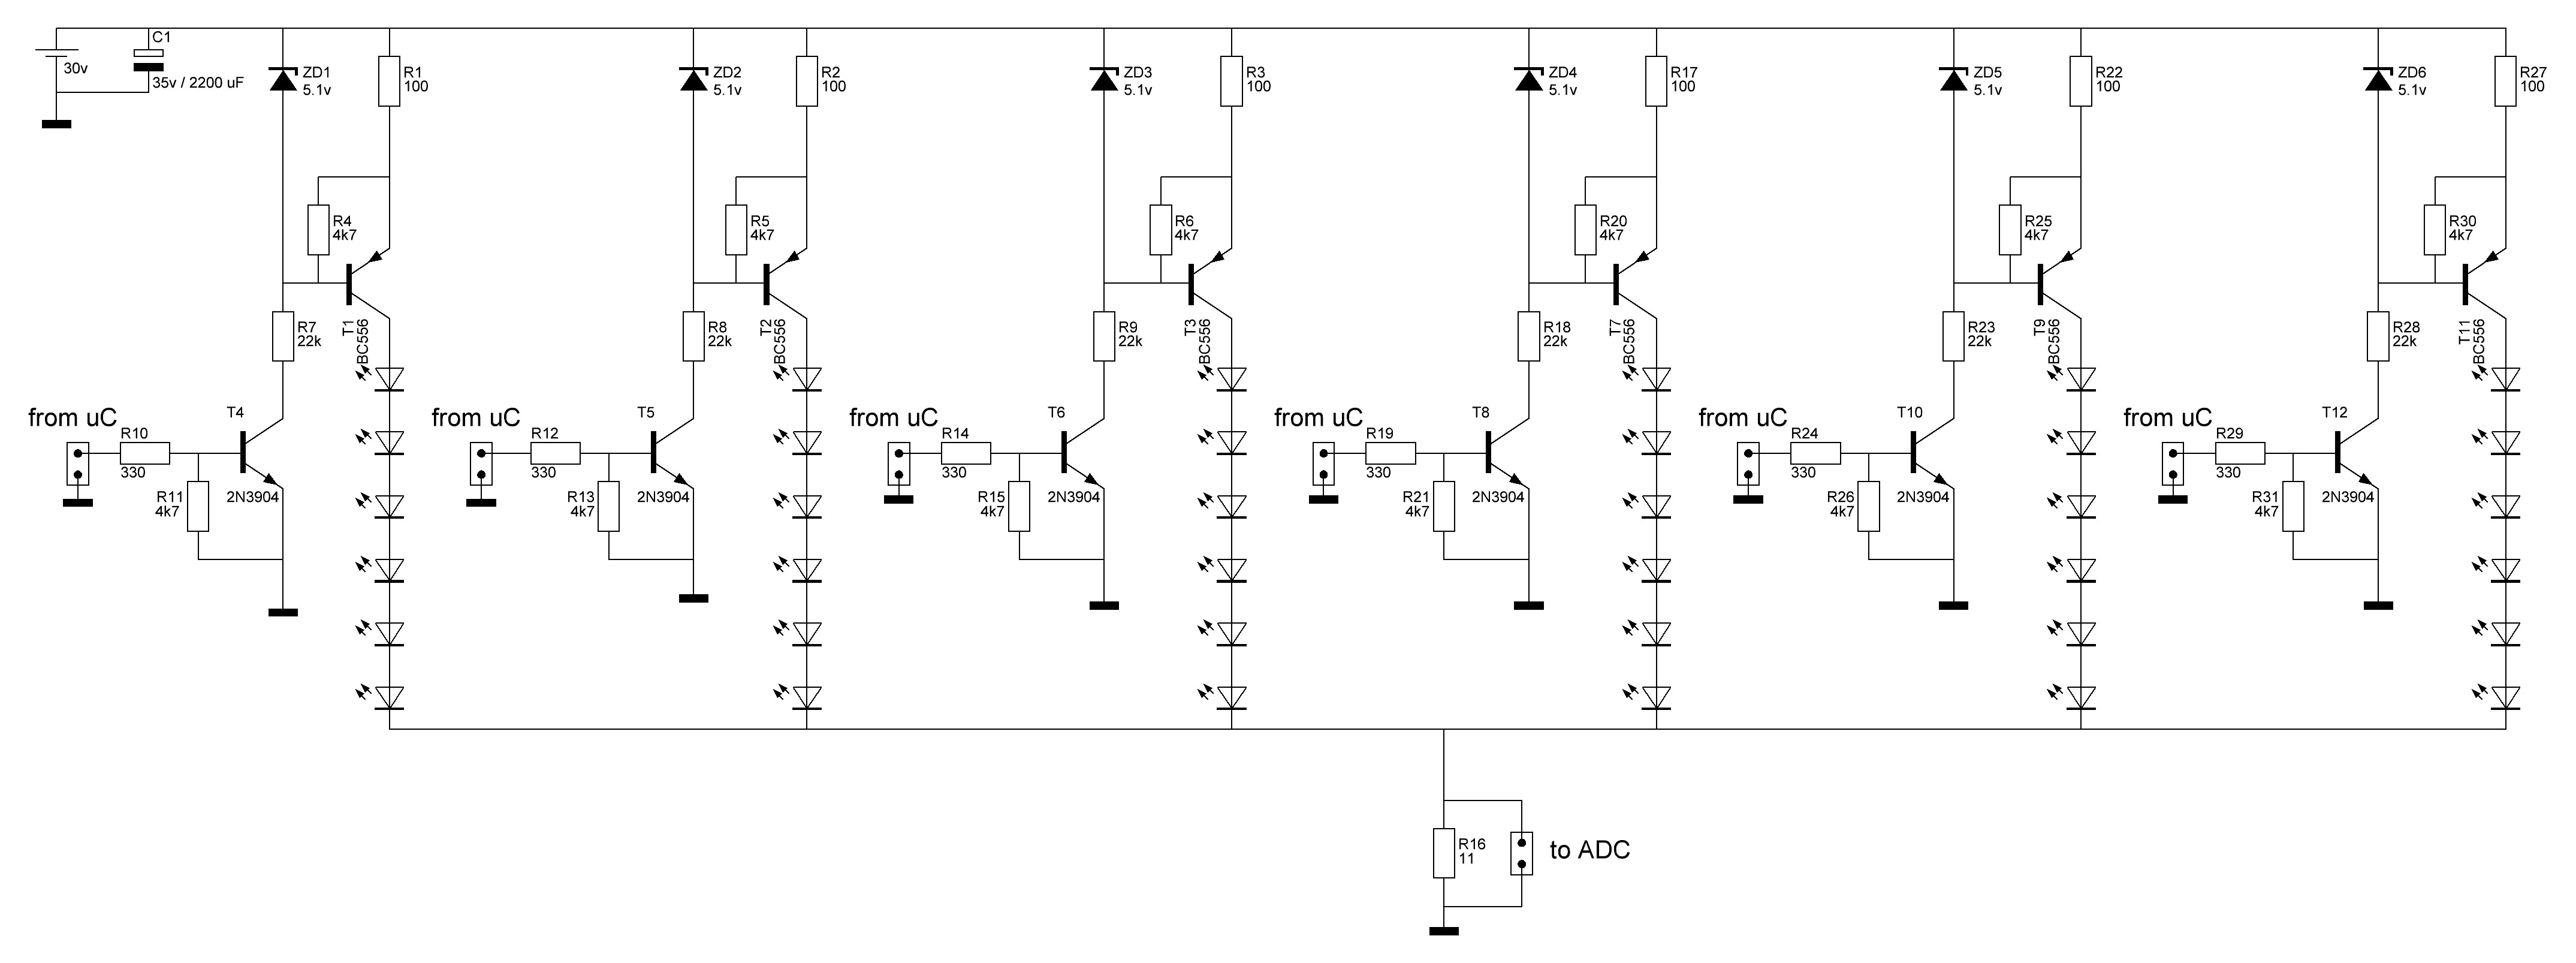
\includegraphics[angle=90,width=\textwidth,height=.9\textheight,keepaspectratio]{chapters/appendix/dc-test-bed/dc-test-bed-schematic.jpg}
	\caption{Schematic of the DC testbed, to modulate six individual LEDs and measure the combined current.}
	\label{fig:dc-test-bed-schematic}
\end{figure}

